\documentclass[a4paper, article]{article}
\usepackage[utf8]{inputenc}
\usepackage[a4paper,total={6in, 8in}]{geometry}
\usepackage[brazil]{babel}
\usepackage{graphicx}
\usepackage{setspace}
\onehalfspacing

\begin{document} 
    \title{\vspace{-3cm}Atividade de Seminários II}
    \author{Luiz Junio Veloso Dos Santos\\ Ciência da Computação}
    \date{Setembro de 2018}
    \maketitle

    \begin{enumerate}
        {\large \item \textbf{Jantar dos Filósofos:}}\\
            \begin{figure}[h]
                \centering
                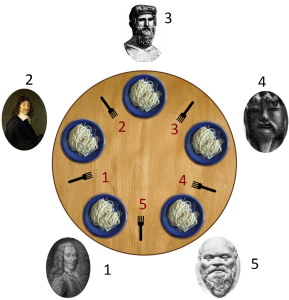
\includegraphics[width=5cm]{Imagens/jdf.png}
            \end{figure}
            \begin{enumerate}
                {\large \item \textbf{O que é?}}\\
                O jantar dos filósofos é um tipo de problema clássico na Computação, criado
                em 1965 por Edsger Dijkstra que diz:\\
                \
                Imagine que existem 5 filósofos que só fazem 2 coisas na vida, comer e pensar.
                Um dia esses filósofos dividem uma mesa redonda com 5 lugares, cada lugar pertence
                a um filósofo. No centro da mesa encontra-se uma tigela de macarrão e 
                estão 5 garfos na mesa, um para cada filósofo, contudo cada filósofo só come com 2
                garfos.\\
                Quando um filósofo pensa, ele não interage com os seus colegas. Com o passar do tempo,
                cada filósofo fica com fome e tenta apanhar os dois garfos que estão mais próximos
                (Os que estão ou à esquerda ou à direita). O filósofo apenas pode apanhar um garfo
                de cada vez, e por isso não pode apanhar um garfo se este estiver na mão do vizinho.\\
                Quando um filósofo esfomeado tiver 2 garfos ao mesmo tempo, ele come sem largar os garfos.
                Apenas quando termina de comer que ele deixa os garfos novamente sobre a mesa, e em seguida
                volta a pensar novamente.\\ 

                O problema é encontrar uma forma que nenhum filósofo morra de fome.

                \item Uma solução:\\
                    Para isso, o jantar será modelado usando uma thread para representar cada filósofo 
                    e usaremos semáforos para representar cada garfo. Quando um filósofo tenta agarrar 
                    um garfo executa uma operação wait no semáforo, quando o filósofo larga o garfo 
                    executa uma operação signal nesse mesmo semáforo. Cada filósofo (thread) vai seguir
                    o algoritmo, ou seja, todos fazem as mesmas ações. Como deve estar já o leitor a pensar,
                    o facto de seguirem o mesmo algoritmo pode dar azo à situação de deadlock, dai a utilização
                    das primitivas de sincronização wait e signal. Uma outra possibilidade de deadlock seria 
                    o facto de mais do que um filósofo ficar com fome ao mesmo tempo, os filósofos famintos 
                    tentariam agarrar os garfos ao mesmo tempo. Isto é outro ponto que uma solução satisfatória 
                    terá que ter em atenção, devendo ser salvaguardado o facto de um filósofo não morrer à fome. 
                    Devemos recordar o leitor que uma solução livre de deadlock não elimina necessariamente
                    a possibilidade de um filósofo morrer esfomeado.


            \end{enumerate}
        \item Problema Produtor-Consumidor:
    \end{enumerate}


\end{document}
